\documentclass[../xlapes02]{subfiles}
\begin{document}
    \chapter{Stock Portfolio Allocation}\label{ch:stock-portfolio-allocation}
    In this chapter, our primary objective is to present the methodology we used to tackle the Reinforcement Learning problem, with a specific focus on the Portfolio Allocation task.\ We will provide a detailed explanation of the entire pipeline~\cref{fig:pipeline}, starting from the \emph{Data Engineering Step}.\ In this step, the data is prepared for use in reinforcement learning.\ This involves collecting raw data from the various sources, transforming the data into features suitable for reinforcement learning, and splitting the dataset into training and testing sets~\cref{sec:data-engineering}.\ Then go on the \emph{Environment Modeling Step}.\ This step involves configuring the environment in which the RL model will operate, including setting up the state and action spaces and defining the reward function, this is described in~\cref{sec:environment-modeling}.\ In the next chapter we also explain the \emph{Agent Layer}, where the model itself is developed here.\ It includes training the model on the training set, evaluating the model's performance on the testing set, fine-tuning the model's hyperparameters to optimize its performance, and conducting robustness testing on unseen data multiple times to ensure that the model can generalize well, this is discussed in~\cref{ch:experiments-and-results}.

    \begin{figure}[ht!]
        \centering
        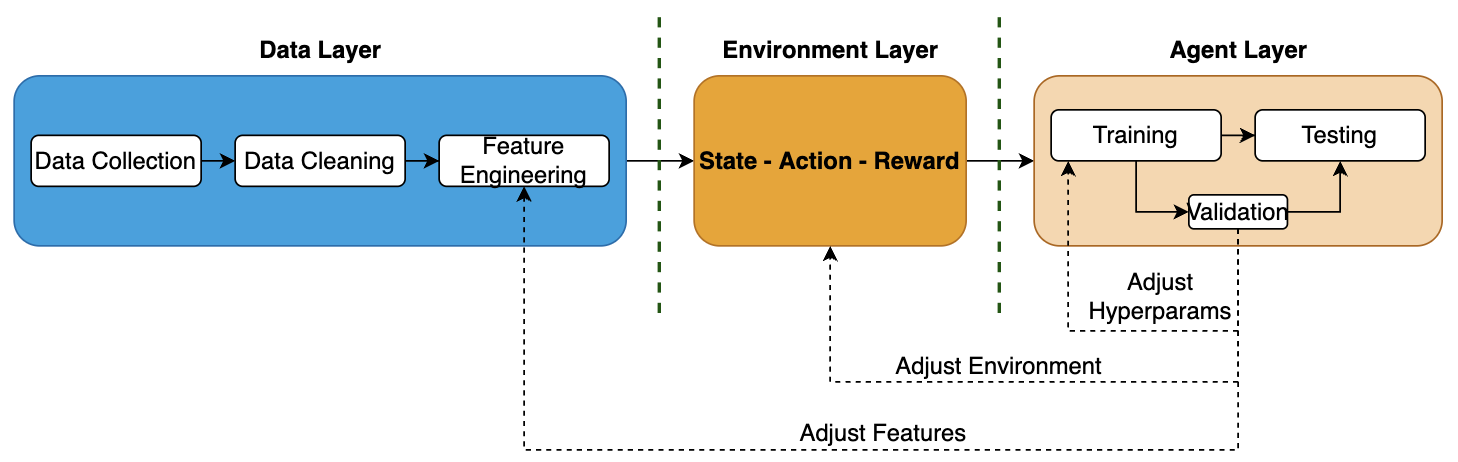
\includegraphics[width=0.8\textwidth]{./image/pipeline}
        \caption{The pipeline for solving the RL problem in the stock market~\cite{liu2022finrlmeta}}
        \label{fig:pipeline}
    \end{figure}


    \section{Data Engineering}\label{sec:data-engineering}
    Data engineering is critical in AI to ensure quality, preparation, integration, scalability, governance, and performance optimization of models.\ It involves cleaning, and transforming data for training an accurate model.\ In this section, we describe our approach to data engineering used for Portfolio Management by first defining the data collection~\cref{subsec:data-collection}, data cleaning~\cref{subsec:data-cleaning}, feature engineering~\cref{subsec:feature-engineering} and dataset splitting~\cref{subsec:dataset-splitting}.

    \subsection{Data Collection}\label{subsec:data-collection}
    Raw data was gathered from these sources:
    \begin{itemize}
        \label{item:data-sources}
        \item Yahoo Finance: \url{https://finance.yahoo.com/}
        \item Financial Modeling Prep: \url{https://financialmodelingprep.com/}
        \item TraidingView: \url{https://www.tradingview.com/}
    \end{itemize}
    these sources provide financial data for 60000+ tickers, with a history of over 30 years.

    We focus on tickers (companies) from Dow Jones Industrial Average (DJIA), which includes 30 companies.\ More about which companies included in DJIA, you can see~\cite{enwiki:1141766585}.

    \subsection{Data Cleaning}\label{subsec:data-cleaning}
    We use the following company data in our datasets: prices, financial statements and technical indicators.\ Prices are used to calculate earnings, financial statements are used to calculate fundamentals.\ Fundamental indicators and technical analysis indicators are used for feature engineering.\ Data cleaning is done by removing rows with missing values.\ Missing values are replaced by the average of the column.\ If data is completely missing on a date, all rows up to that next date are removed for the other companies.\ This can happen mostly for companies that are not listed in any time period.\ Data cleaning is performed for all data sets.

    \subsection{Feature Engineering}\label{subsec:feature-engineering}
    In this subsection, we describe our approach to feature engineering which we divide into three parts: \emph{Fundamental Analysis}, described in~\cref{subsubsec:fundamental-analysis}, \emph{Technical Analysis}, described in~\cref{subsubsec:technical-analysis}, and \emph{Combined Fundamental and Technical Analysis} is described in~\cref{subsubsec:combined-fundamental-and-technical-analysis}.\ The datasets comprises of additional attributes such as candlestick patterns (price) and volumes, which are not discussed in this subsection.

    \subsubsection{Fundamental Analysis}\label{subsubsec:fundamental-analysis}
    First features that we used for our datasets are fundamental information about companies.\ This type of data is essentially the key and crucial information that is utilized to analyze the financial well-being, performance and worth of a company or asset.\ It encompasses information regarding the financial statements, business operations, management team, industry and economic backdrop of a company.\ Investors, analysts and financial experts commonly use fundamental data to make informed investment decisions and evaluate the inherent value of an asset.\ The subsequent text outlines the features that were incorporated into our dataset.\ There also exists a plethora of other fundamental features that can be used, but we have chosen to focus on the following features, with the theoretical concepts sourced from~\cite{investopedia}:

    \paragraph{Operating Margin}\label{par:operating-margin}
    The Operating Margin represents how efficiently a company is able to generate profit through its core operations.\ It is expressed on a per-sale basis after accounting for variable costs but before paying any interest or taxes (EBIT). Higher margins are considered better than lower margins and can be compared between similar competitors but not across different industries.\ To calculate the operating margin, divide operating income (earnings) by sales (revenues):
    \begin{equation}
        \label{eq:operating-margin}
        Operating\ Margin=\frac{Operating\ Income}{Net\ Sales}
    \end{equation}
    where $Operating\ Income$ refers to the adjusted revenue of a company after all expenses of operation and depreciation are subtracted.\ Expenses of operation or operating expenses are simply the costs incurred in order to keep the business running. $Net\ Sales$ may be defined as money paid by customers.\ Sales are a company's core revenue for a given period.\ Operating margin, expressed as a percentage, indicates the earnings generated from each dollar of sales after accounting for direct costs.\ Higher margins mean more profit from each sale.

    \paragraph{Net Profit Margin}\label{par:net-profit-margin}
    The Net Profit Margin is a profitability ratio that measures a company's ability to generate income after all expenses and taxes have been paid $Net\ Income$.\ It is calculated by dividing a company's $Net\ Income$, by its $Total\ Revenue$.\ The $Net\ Profit\ Margin$ is a measure of how much of each dollar of revenue is left over after all expenses and taxes have been paid.\ It is a useful metric for comparing the profitability of different companies in the same industry.\ The higher the net profit margin, the more profitable a company is.\ The net profit margin is calculated as follows:
    \begin{equation}
        \label{eq:net-profit-margin}
        \begin{split}
            Net\ Profit\ Margin&=\frac{Net\ Income}{Total\ Revenue}\\
        \end{split}
    \end{equation}

    \paragraph{Return On Assets}\label{par:return-on-assets}
    Return on assets (ROA) is a measure of profitability that calculates how much profit a company makes with the money it has invested.\ It is calculated by dividing a company's $Net\ Income$ by its $Total\ Assets$.\ The higher the ROA, the more profitable a company is.\ The ROA is calculated as follows:
    \begin{equation}
        \label{eq:return-on-assets}
        \begin{split}
            Return\ On\ Assets&=\frac{Net\ Income}{Total\ Assets}\\
        \end{split}
    \end{equation}

    \paragraph{Return On Equity}\label{par:return-on-equity}
    Return on equity (ROE) is a measure of profitability that calculates how much profit a company makes with the money shareholders have invested.\ It is calculated by dividing a company's $Net\ Income$ by its $Average\ Shareholders'\ Equity$.\ The higher the ROE, the more profitable a company is.\ The ROE is calculated as follows:
    \begin{equation}
        \label{eq:return-on-equity}
        \begin{split}
            Return\ On\ Equity&=\frac{Net\ Income}{Average\ Shareholders'\ Equity}\\
        \end{split}
    \end{equation}

    \paragraph{Current Ratio}\label{par:current-ratio}
    The current ratio is a liquidity ratio that measures a company's ability to pay short-term and long-term obligations.\ It is calculated by dividing a company's $Current\ Assets$ by its $Current\ Liabilities$.\ The higher the current ratio, the more capable a company is of paying its short-term and long-term obligations.\ The current ratio is calculated as follows:
    \begin{equation}
        \label{eq:current-ratio}
        \begin{split}
            Current\ Ratio&=\frac{Current\ Assets}{Current\ Liabilities}\\
        \end{split}
    \end{equation}
    where $Current\ Assets$ is $Cash\&Equivalent+Short\ Term\ Investments+Account\ Receivable+Inventory$.\ If the $Current Ratio < 1$ that is a sign of financial distress, and the company could be unable to pay its short-term and long-term obligations.\ On the other hand, if the $Current Ratio$ is too high, it could be a sign that the company is not using its assets efficiently.

    \paragraph{Quick Ratio}\label{par:quick-ratio}
    The quick ratio is a liquidity ratio that measures a company's ability to pay short-term obligations.\ It is calculated by dividing a company's $Quick\ Assets$ by its $Current\ Liabilities$.\ The higher the quick ratio, the more capable a company is of paying its short-term obligations.\ The quick ratio is calculated as follows:
    \begin{equation}
        \label{eq:quick-ratio}
        \begin{split}
            Quick\ Ratio&=\frac{Quick\ Assets}{Current\ Liabilities}\\
        \end{split}
    \end{equation}
    where $Quick\ Ratio$ is $Cash\&Equivalents+Marketable\ Securities+Net\ Accounts\ Receivable$.\ If the company would have a $Quick Ratio < 1$, it would be a sign of financial distress, and the company would be unable to pay its short-term obligations.

    \paragraph{Cash Ratio}\label{par:cash-ratio}
    The cash ratio is a liquidity ratio that measures a company's ability to pay short-term obligations.\ It is calculated by dividing a company's $Cash\&Equivalents$ by its $Current\ Liabilities$.\ The higher the cash ratio, the more capable a company is of paying its short-term obligations.\ The cash ratio is calculated as follows:
    \begin{equation}
        \label{eq:cash-ratio}
        \begin{split}
            Cash\ Ratio&=\frac{Cash\&Equivalent}{Current\ Liabilities}\\
        \end{split}
    \end{equation}

    \paragraph{Inventory Turnover}\label{par:inventory-turnover}
    The inventory turnover ratio is a measure of how efficiently a company is managing its inventory.\ It is calculated by dividing a company's $COGS$ by its $Average\ Value\ of\ Inventory$.\ The higher the inventory turnover ratio, the more efficiently a company is managing its inventory.\ The inventory turnover ratio is calculated as follows:
    \begin{equation}
        \label{eq:inventory-turnover}
        \begin{split}
            Inventory\ Turnover&=\frac{COGS}{Average\ Value\ of\ Inventory}\\
        \end{split}
    \end{equation}
    where $COGS$ is an acronym for Cost of Goods Sold, which is also known as the cost of sales.\ To calculate inventory turnover, analysts use COGS instead of sales because inventory is valued at cost.\ Some companies may use sales instead of COGS, which can inflate the ratio.

    \paragraph{Receivables Turnover}\label{par:receivables-turnover}
    The receivables turnover ratio is a measure of how efficiently a company is managing its accounts receivable.\ It is calculated by dividing a company's $Net\ Credit\ Sales$ by its $Average\ Accounts\ Receivable$.\ The higher the receivables turnover ratio, the more efficiently a company is managing its accounts receivable.\ The receivables turnover ratio is calculated as follows:
    \begin{equation}
        \label{eq:receivables-turnover}
        \begin{split}
            Receivables\ Turnover&=\frac{Net\ Credit\ Sales}{Average\ Accounts\ Receivable}\\
        \end{split}
    \end{equation}
    where $Net\ Credit\ Sales$ is the total sales minus the cash sales.\ The receivables turnover ratio measures a company's ability to collect accounts receivable.\ A low ratio suggests difficulty collecting payments, while a high ratio may indicate efficient collection, but may also suggest lost sales due to not extending credit long enough.

    \paragraph{Payables Turnover}\label{par:payables-turnover}
    The accounts payable turnover ratio is a short-term liquidity measure used to quantify the rate at which a company pays off its suppliers.\ Accounts payable turnover shows how many times a company pays off its accounts payable during a period.\ It is calculated by dividing a company's total suply purchases by its average accounts payable.\ The higher the payables turnover ratio, the more efficiently a company is managing its accounts payable.\ The payables turnover ratio is calculated as follows:
    \begin{equation}
        \label{eq:payables-turnover}
        \begin{split}
            Payables\ Turnover&=\frac{TSP}{(BAP+EAP)/2}\\
        \end{split}
    \end{equation}
    where $TSP$ is the total supply purchase, $BAP$ is the beginning accounts payable, and $EAP$ is the ending accounts payable.\ If the payables turnover ratio is too low, it could be a sign that company has trouble paying its suppliers.\ If the payables turnover ratio is too high, it could be a sign that the company is not using its assets efficiently.

    \paragraph{Debt Ratio}\label{par:debt-ratio}
    The debt ratio is a measure of a company's financial leverage.\ It is calculated by dividing a company's $Total\ Liabilities$ by its $Total\ Assets$.\ The higher the debt ratio, the more debt a company is using to finance its assets.\ The debt ratio is calculated as follows:
    \begin{equation}
        \label{eq:debt-ratio}
        \begin{split}
            Debt\ Ratio&=\frac{Traditional\ Debt+(Accounts\ Payable+Taxes\ Payable)}{Total Assets}\\
        \end{split}
    \end{equation}
    A lower debt ratio is preferable.\ A Debt Ratio greater than 1.0 implies that a company has more debt than assets, whereas a Debt Ratio less than 1 indicates that a company has more assets than debt.

    \paragraph{Debt Equity Ratio}\label{par:debt-equity-ratio}
    The Debt to Equity Ratio (D/E) is a measure of a company's financial leverage.\ It is calculated by dividing a company's $Total\ Liabilities$ by its $Total\ Equity$.\ The higher the debt equity ratio, the more debt a company is using to finance its assets.\ The debt equity ratio is calculated as follows:
    \begin{equation}
        \label{eq:debt-equity-ratio}
        \begin{split}
            Debt\ Equity\ Ratio&=\frac{Total\ Liabilities}{Total\ Equity}\\
        \end{split}
    \end{equation}
    where $Total\ Liabilities$ are $Traditional\ Debt+(Accounts\ Payable+Taxes\ Payable)$.\ A lower $Debt\ Equity\ Ratio$ is preferable.

    \paragraph{Price Earnings Ratio}\label{par:price-earnings-ratio}
    The Price Earnings Ratio (P/E) is a measure of a company's value relative to its earnings.\ It is calculated by dividing a company's $Stock\ Price$ by its $Earnings\ per\ Share$.\ The higher the price earnings ratio, the more expensive a company's stock is relative to its earnings.\ The price earnings ratio is calculated as follows:
    \begin{equation}
        \label{eq:price-earnings-ratio}
        \begin{split}
            Price\ Earnings\ Ratio&=\frac{Stock\ Price}{Earnings\ Per\ Share}\\
        \end{split}
    \end{equation}
    High P/E implies investors anticipate greater future earnings growth compared to low P/E companies.\ A low P/E can signal undervaluation or exceptional performance relative to past trends.

    \paragraph{Price Book Value Ratio}\label{par:price-book-value-ratio}
    The Price Book Value Ratio (P/B) is a measure of a company's value relative to its book value.\ It is calculated by dividing a company's $Stock\ Price$ by its $Book\ Value\ per\ Share$.\ The higher the price book value ratio, the more expensive a company's stock is relative to its book value.\ The price book value ratio is calculated as follows:
    \begin{equation}
        \label{eq:price-book-value-ratio}
        \begin{split}
            Price\ Book\ Value\ Ratio&=\frac{Stock\ Price\ per\ Share}{Book\ Value\ per\ Share}\\
        \end{split}
    \end{equation}
    A low P/B ratio, especially below one, could signal undervaluation where stock price is lower than the value of the company's assets.\ A P/B ratio above one indicates the stock is trading at a premium to book value, potentially overvalued.\ For instance, a P/B ratio of three means the stock trades at three times book value.

    \paragraph{Dividend Yield}\label{par:dividend-yield}
    The dividend yield, expressed as a percentage, is a financial ratio (dividend/price) that shows how much a company pays out in dividends each year relative to its stock price.\ It is calculated by dividing a company's $Annual\ Dividend$ by its $Stock\ Price$.\ It is a measure of a company's profitability.\ The higher the dividend yield, the more profitable a company is.\ The dividend yield is calculated as follows:
    \begin{equation}
        \label{eq:dividend-yield}
        \begin{split}
            Dividend\ Yield&=\frac{Annual\ Dividend}{Stock\ Price}\\
        \end{split}
    \end{equation}

    \subsubsection{Technical Analysis}\label{subsubsec:technical-analysis}
    Technical analysis is a method used in financial markets such as stocks, currencies and commodities to analyse historical price data and identify patterns, trends and signals that can be used to make trading decisions.\ Technical analysis is based on the belief that historical price and volume data can provide insight into future price movements and focuses primarily on the analysis of price charts and other technical indicators.\ In this section we present the technical indicators that we have selected based on the correlation between all indicators.


    Technical indicators are calculated based on historical share price data.\ To calculate these indicators, the Finta framework was used, which provides more than 100 different functions for calculating technical indicators.\ The framework is written in Python and is available on GitHub~\cite{finta}.

    First, we calculate all technical indicators for each stock present in the dataset, followed by determining the correlation matrix between all indicators.\ This matrix comprises the correlation coefficient values between each pair of indicators, which serve as a gauge for measuring the linear correlation between two variables.\ We apply a drop threshold of $0.5$ for the correlation coefficient, implying that if $|\rho| > 0.5$, we discard either the first or second indicator, where $|\rho|$ represents the absolute value of the correlation between the two variables (indicators).\ As the image (correlation matrix) for all indicators is extensive, we only present the correlation matrix of the final indicators (correlation matrix of the uncorrelated indicators), in~\cref{fig:ta_correlation_matrix_uncorrelated_indicators}, that we utilized in the \emph{Technical Analysis Dataset}.\ Since the correlation matrix has symmetry, only the segment above the diagonal is presented.
    \begin{figure}[h]
        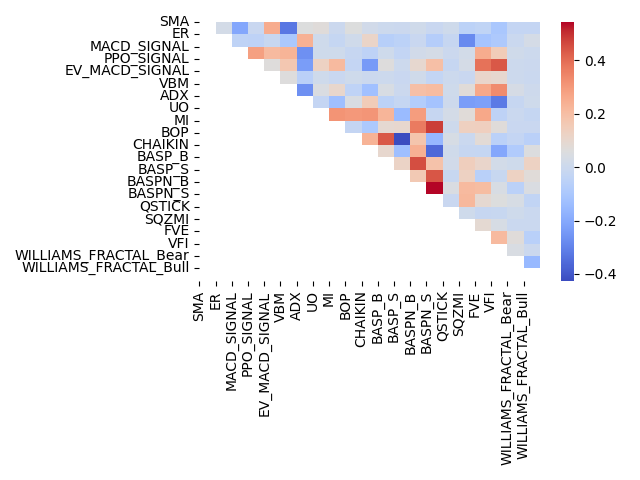
\includegraphics[width=0.95\linewidth]{image/ta_correlation_matrix_uncorrelated_indicators}
        \centering
        \caption{Correlation matrix of technical indicators after removing correlated indicators.}
        \label{fig:ta_correlation_matrix_uncorrelated_indicators}
    \end{figure}

    \subsubsection{Combined Fundamental and Technical Analysis}\label{subsubsec:combined-fundamental-and-technical-analysis}
    Combining datasets is a process in which two or more datasets are merged or joined together to create a new dataset that contains information from both.\ In this case, the combined fundamental and technical analysis involves combining features from both fundamental analysis~\cref{subsubsec:fundamental-analysis} and technical analysis, described in~\cref{subsubsec:technical-analysis}.

    By combining fundamental and technical analysis, we can create a more comprehensive and accurate picture of the market.\ For example, fundamental analysis can help identify undervalued or overvalued assets, while technical analysis can help identify trends and potential buying or selling opportunities.\ The specific features used in the combined analysis can depend on the specific dataset and the reinforcement learning task being performed.\ However, we leave all features from both analysis.

    \subsection{Dataset Splitting}\label{subsec:dataset-splitting}
    Dataset splitting refers to the process of dividing a dataset into two or more subsets to be used for training and testing reinforcement learning models.\ In this particular case, the dataset is a time series data, which means that the order of the data points is important, and the dataset must be split in a way that preserves the temporal ordering.

    The division coefficient of $0.6$ means that $60\%$ of the dataset will be used for training, and $40\%$ will be used for testing.\ This is a common split ratio, but the exact ratio can vary depending on the size and complexity of the dataset, as well as the specific reinforcement learning task being performed.

    In this case, since the dataset consists of daily data and spans a period from 2008-03-20 to 2022-12-16, we can split it based on time.\ The first $60\%$ of the data, starting from the beginning of the dataset on 2008-03-20, will be used for training, and the remaining $40\%$ of the data will be used for testing.\ This ensures that the model is trained on past data and tested on future data, which is a more realistic scenario.

    The training set will be used to train the reinforcement learning model, while the testing set will be used to evaluate its performance.\ By splitting the dataset, we can avoid overfitting, which is when the model memorizes the training data and performs poorly on new, unseen data.\ The testing set provides a way to measure the model's generalization performance on unseen data, which is an important metric for evaluating the model's effectiveness.

    Dataset splitting is an important step in reinforcement learning that helps ensure that the model is trained and tested on different subsets of data.\ In this case, the dataset is split into training and testing sets based on time, with $60\%$ of the data used for training and $40\%$ used for testing.\ This split ensures that the model is evaluated on unseen data and can generalize well to new data.


    %


    \section{Environment Modeling}\label{sec:environment-modeling}
    In the preceding section, we explained the process of creating datasets and selecting features to represent the state of the environment.\ This section delves deeper into the modeling of the entire environment, encompassing the \emph{Action Space}, \emph{State Space}, and \emph{Reward function}.\ The action space is defined as a vector of weights, where each weight denotes the percentage amount that a particular stock is represented in the portfolio.\ This is discussed in detail in~\cref{subsubsec:action-space}.\ The state space is a matrix of $K$ features of each stock ($N$ stocks) that reflects the state of the environment at each time step $t$, as explained in~\cref{subsubsec:state-space}.\ The reward function is employed to calculate the reward for each action taken in the current state at time step $t$, as elaborated in~\cref{subsubsec:reward-function-portfolio}.\ The objective of the agent is to maximize the reward by selecting the best action/weights for each state, which involves reallocating the stock weights in the portfolio.\ In other words, the agent aims to determine the optimal weights for each stock in the portfolio at a particular time step $t$ to obtain maximum portfolio appreciation.\ The ~\cref{fig:state_agent_weights} illustrates how the agent generates the weights for the portfolio.

    \begin{figure}[ht!]
        \centering
        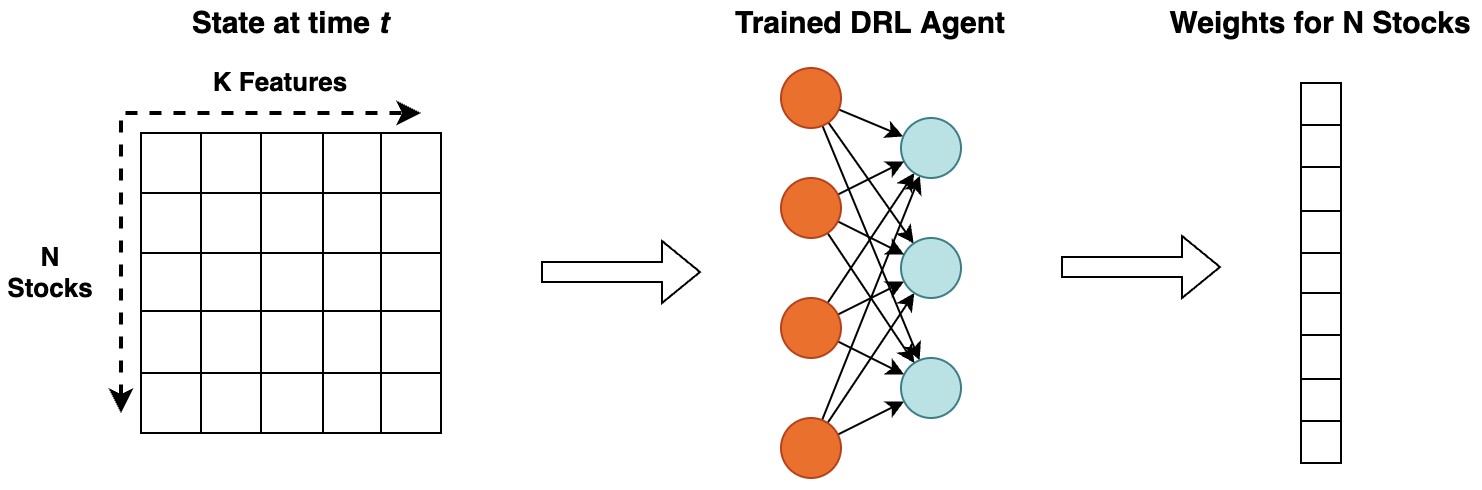
\includegraphics[width=0.8\textwidth]{./image/state_agent_weightss}
        \caption{How the agent produces the weights for the portfolio~\cite{finrl-portfolio-allocation-2020}.}
        \label{fig:state_agent_weights}
    \end{figure}

    \subsection{Portfolio Management Task}\label{subsec:portfolio-management-task}
    Portfolio allocation or management refers to the process of selecting and distributing investments in a way that meets the investor's goals and risk tolerance.\ It involves diversifying the portfolio across different asset classes, such as stocks, bonds, and real estate, to reduce risk and increase returns.\ In our thesis we focus on diversifying the capital between \textbf{$N$ stocks}, where $N$ is the number of stocks in the portfolio.\ The ultimate goal of portfolio management is to maximize the returns while minimizing the risk for the investor~\cite{finrl-portfolio-allocation-2020}.

    %

    \subsubsection{Risk of Portfolio}\label{subsubsec:risk-of-portfolio}
    Risk is evaluated as the variance of the portfolio returns, according to~\cref{eq:risk}.
    \begin{equation}
        \label{eq:risk}
        \text{Risk}(t)=\text{Var}(\rho(t))=\text{Var}(\bm{w}(t)^\top \bm{y}(t) - 1)
    \end{equation}
    where $\rho(t)$ is the return of portfolio at time step $t$ and is further explained in~\cref{subsubsec:reward-function-portfolio} with relation to \emph{Reward function}. $\bm{w}(t)$ is the weight vector of the portfolio at time step $t$, and $\bm{y}(t)$ is the vector of stock prices change at time step $t$ relative to time step $t-1$, according to~\cref{eq:price-relative-vector}.

    %

    \subsubsection{State and Observation Space}\label{subsubsec:state-space}
    In the context of portfolio management, the \emph{State Space} and \emph{Observation space} refer to the same set of variables.\ The state space is a matrix with dimensions $N\times K$, where $N$ represents the number of risky assets, or stocks, and $K$ represents the number of features used to describe the environment.\ These features were discussed in detail in the previous section~\cref{sec:data-engineering}, and consist of fundamental or technical indicators that describe the current condition of each stock at a specific time step $t$.\ In our case, the time step is defined as one day, so we use \textbf{daily data} representing one day of stock market activity.

    %

    \subsubsection{Action Space}\label{subsubsec:action-space}
    The action space for a portfolio allocation agent is a vector of $N+1$ values, which represents the weights of $N$ stocks and weight of cash (How much is each stock represented in portfolio).\ The reason for including a weight of cash in the action space is that sometimes investors do not want to invest all of their capital and prefer to keep some cash as a reserve for future trades.\ The action provided by the agent is a vector of values \textbf{bounded between 0 and 1}.

    The action vector is then normalized using the \emph{softmax function}.\ The softmax function converts the original vector of real values into a new vector of real values that fall within the range of 0 to 1, and all values summed to 1.\ This allows for a more intuitive representation of the weights and ensures that the weights always add up to 1~\cite{finrl-portfolio-allocation-2020}.

    Action vector is provided by an agent at time step $t$ and is defined as follows:
    \begin{equation}
        \label{eq:action-vector}
        \bm{a}(t) = [a_1(t), a_2(t), \ldots, a_N(t), a_{cash}(t)]
    \end{equation}
    where $a_i(t)$ is the value before normalization for stock $i$ at time step $t$ and $a_{cash}(t)$ is for cash at time step $t$.\ The weights vector $\bm{w}(t)$ is defined as follows:
    \begin{equation}
        \label{eq:weights-vector}
        \begin{split}
            \bm{w}(t) &= \text{softmax}(\bm{a}(t)) = \frac{\exp(\bm{a}(t))}{\sum_{i=1}^{N}\exp(a_i(t))} \\
            &= [w_1(t), w_2(t), \ldots, w_N(t), w_{cash}(t)]
        \end{split}
    \end{equation}
    where $w_i(t)$ is the normalized weight for stock $i$ at time step $t$ and $w_{cash}(t)$ is for cash at time step $t$.\ All weights vectors must summed to 1, and it directly implies the second constrained that each weight must be bounded between 0 and 1:
    \begin{equation}
        \label{eq:equation-constraint}
        \sum_{i=1}^{N}w_i(t)=1,\quad w_i(t)\in[0,1],\quad t=1,\ldots,T
    \end{equation}

    %

    \subsubsection{Reward Function}\label{subsubsec:reward-function-portfolio}
    The reward function represents the change in the value of the portfolio from one time step to the next.\ First we need to define \emph{Price Relative Vector} $\bm{y}(t) \in \mathbb{R}^N$:
    \begin{equation}
        \label{eq:price-relative-vector}
        \begin{split}
            \bm{y}(t)=\left[\frac{p_1(t)}{p_1(t-1)}, \frac{p_2(t)}{p_2(t-1)}, \cdots, \frac{p_N(t)}{p_N(t-1)}, 1\right]\text{ , for }t=1,\ldots,T
        \end{split}
    \end{equation}
    where the $p_i(t)$ is the price of risky asset (stock) at time step $t$, and $\frac{p_i(t)}{p_i(t-1)}$ represents the relative change in price from one-time slot to the next of stock $i$, we incorporate into the vector also the change of cash, which is constant value $1$ (we assume that cash value do not change its value).

    Now we can define our \textbf{Reward function} as rate of portfolio return:
    \begin{equation}
        \label{eq:rate-of-portfolio-return}
        \rho(t)=\bm{w}(t-1)^\top\bm{y}(t)-1\text{ , for }t=1,\ldots,T
    \end{equation}
    The reward function measures the change in the portfolio's value between consecutive time steps.\ We assume that there are no transaction costs associated with each operation, as these can vary depending on the broker.\ Additionally, we don't factor in any dividends.\ Instead, the reward is solely based on the change in the value of each stock.

    Lastly we defined the \emph{portfolio value} $v(t) \in \mathbb{R}$ at time step $t$.\ First let the $v(0)$ be an initial capital, then for $t=1,\ldots,T$ is portfolio value defined as follows:
    \begin{equation}
        \label{eq:portfolio-value}
        \begin{split}
            v(t) &=v(0)\prod_{\tau=1}^{t}\left[\rho(\tau)+1\right]\\
            &=v(t-1)(\rho(t)+1)
            \text{ , for }t=1,\ldots,T
        \end{split}
    \end{equation}
    where $\rho(t)$ is change in portfolio value (\emph{Reward}) at time step $t$.

\end{document}
